

\section{INT8 Attention for Training}

Low-bit quantization attention works, such as FlashAttention3 and SageAttention, are only for inference. In this section, we propose an \texttt{INT8} attention for training, named \texttt{SageBwd}, which quantizes six of seven matrix multiplications in attention to \texttt{INT8}, achieving no performance degradation in fine-tuning tasks.
Besides, we implement both \texttt{INT8} \texttt{SageBwd} and \texttt{FP8} \texttt{SageBwd} and conduct comparison experiments, proving \texttt{INT8} \texttt{SageBwd} is superior to \texttt{FP8} \texttt{SageBwd} in Section~\ref{sec:in8_vs_fp8_sagebwd}.

\begin{algorithm}[H]
    \small
    \caption{Forward pass of the \texttt{8-bit} attention.}
    \label{alg:int8_train_fwd} 
    % \setlength{\textfloatsep}{-10pt}
    \begin{algorithmic}[1]
    \STATE {\bfseries Input:} {\texttt{FP16} matrices $Q, K, V \in \mathbb{R}^{N \times d}$, and block size $B_q, B_{kv}$.}

    \STATE $K_m = {\rm mean}(K); ~~ K\gets K-K_m$ ; \annotate{// Smooth-k technique.}
    
    \STATE Divide $Q$ to $T_m = {N}/{B_q}$ blocks $\{\vQ_i\}$; divide $K$, and $V$ to $T_n = {N}/{B_{kv}}$ blocks $\{\vK_i\}$, $\{\vV_i\}$ ;  

    \STATE {\bfseries Quantization:} \jt{$\{\mathbf{s_Q}, \hat \vQ_i\} = \{\psi (\vQ_i)\}$, ~~ $\{\mathbf{s_K}, \hat \vK_i\} = \{\psi (\vK_i^\top)\}$, ~~$\{\mathbf{s_V}, \hat \vV_i\} = \{\psi (\vV_i)\}$} ; \annotate{// Per-block.}

    \FOR {$i=1$ {\bfseries to} $T_m$}

    \STATE $\vO_i \in \mathbb{R}^{B_q\times D}= (0)$, ~~ $\mathbf{L}_i \in \mathbb{R}^{B_q} = (0),~~ m_i \in \mathbb{R}^{B_{kv}} = (0)$ ;

        \FOR {$j$ in [1, $T_n$]} 

            \STATE \jt{$\vS_{ij} = \texttt{MM} (\hat \vQ_i, \hat \vK_j) \times \mathbf{s_Q} \times \mathbf{s_K}$} ;  

            \STATE $m_{ij} = \mathrm{max}(m_{i,j-1}, \mathrm{rowmax}(\vS_{ij}))$, $\widetilde \vP_{ij} = \mathrm{exp}(\vS_{ij} - m_{ij})$, $l_{ij} = e^{m_{i,j-1}-m_{ij}} l_{i,j-1} + \mathrm{rowsum}(\widetilde \vP_{ij})$;

            \STATE \jt{$\mathbf{s_P} = \mathrm{exp}(\rowmax(\vS_{ij}) - m_{ij}) / 127$, ~~ $\mathbf{\hat \vP}_{ij} = \widetilde \vP_{ij} / \mathbf{s_P}$} ; \annotate{// Per-token quantization.}

            \STATE $\vO_{ij} = \mathrm{diag}(e^{m_{i,j-1}-m_{ij}}) \vO_{i,j-1} + \jt{\texttt{MM}(\hat \vP_{ij}, \hat \vV_j) \times \mathbf{s_{P}} \times \mathbf{s_V}}$
        
        \ENDFOR
        \STATE $\vO_i = \mathrm{diag}(l_{i,T_n}) ^{-1} \vO_{i,T_n}$ ;  %~~~ Write $\vO_i$ ;  
        \STATE $\mathbf{L}_i = m_{i, T_n} + \mathrm{log}(l_{i, T_n})$ ; %~~~ Write $\mathbf{L}_i$ ;
    \ENDFOR
    
    \STATE \textbf{return} $O = \{\vO_i\}$, $L = \{\mathbf{L}_i\}$ ;
    \end{algorithmic}
    \vspace{-.15em}
\end{algorithm}

\subsection{Forward}
There are two matrix multiplications in the forward pass of attention:
\begin{align}
    \vS = \vQ\vK^\top,~~ \vO = \vP \vV
\end{align}
\textbf{Per-token quantization for P.} Following SageAttention~\citep{2024sageattention}, we apply smoothing K and per-block \texttt{INT8} quantization for the $\vQ\vK^\top$. However, for the $\widetilde \vP \vV$, a static per-block \texttt{INT8} quantization with a static scale factor of $\mathsf{1/127}$ for $\widetilde \vP$ is inaccurate~\citep{2024sageattention}. Fortunately, we find applying per-token \texttt{INT8} quantization for $\widetilde \vP \vV$ and per-block \texttt{INT8} quantization for $\vV$ can enhance the attention accuracy. 
Furthermore, we eliminate the need for explicit $\max$ operations on $\vP$ by reusing both global and local maximum values from the online softmax computation (Line 9 in Algorithm~\ref{alg:int8_train_fwd}).
The algorithm for the forward is shown in Algorithm~\ref{alg:int8_train_fwd}.


Given our extensive use of \texttt{INT8} per-block quantization in trainable attention, we formalize the process as follows. For each FlashAttention block $\mathbf{X}$, the quantization process $\mathbf{s_X}, \mathbf{\hat X} = \psi(\mathbf{X})$ can be formulated as:
\begin{align}
    \mathbf{s_X} = \max(|\mathbf{X}|)/127, ~~~ \mathbf{\hat X}=\mathbf{X}/\mathbf{s_X}
\end{align}
\begin{algorithm}[H]
    \small
    \caption{Backward pass of the \texttt{8-bit} attention.}
    \label{alg:int8_train_bwd} 
    % \setlength{\textfloatsep}{-10pt}
    \begin{algorithmic}[1]
    \STATE {\bfseries Input:} \jt{$\{\mathbf{s_Q}, \hat \vQ_i\}, \{\mathbf{s_K}, \hat \vK_i\}, \{\mathbf{s_V}, \hat \vV_i\}$}, $K_m$, $O$, $\{\mathbf{L}_i\}$ from forward, $dO \in \mathbb{R}^{N \times d}$, block size $B_q, B_{kv}$ ; 

    \STATE $D = \mathrm{rowsum}(dO \circ O)$, ~~ divide $D$ to $T_m = {N}/{B_q}$ blocks $\{\mathbf{D}_i\}$; 

    \FOR {$j=1$ {\bfseries to} $T_n$}

        \FOR {$i$ in [1, $T_m$]} 

            \STATE \jt{$\vS_{ij} = \texttt{MM} (\hat \vQ_i, \hat \vK_j) \times \mathbf{s_Q} \times \mathbf{s_K}$} ;  ~~~~~$\vP_{ij} = \mathrm{exp}(\vS_{ij} - \mathbf{L}_{i})$ ;

            \STATE \jt{$\mathbf{s_P}, \hat \vP_{ij} = \psi(\vP_{ij})$, ~~ $\mathbf{s_{dO}}, \hat \vdO_{i} = \psi(\vdO_{i})$} ; ~\annotate{// \texttt{INT8} per-block quantization.}

            \STATE $\vdV_j \leftarrow \vdV_j + \jt{\texttt{MM}(\hat \vP_{ij}^\top, \hat \vdO_{i}) \times \mathbf{s_P} \times \mathbf{s_{dO}}}$ ;

            \STATE $\vdP_{ij} = \texttt{MM}(\vdO, \vV_j^\top)$ ;  ~\annotate{// Keep in \texttt{FP16}.}

            \STATE $\vdS_{ij} = \vP_{ij} \circ (\vdP_{ij} - \mathbf{D}_i)$ ; ~~~~~\jt{$\mathbf{s_{dS}}, \hat \vdS_{ij} = \psi(\vdS_{ij})$} ; ~\annotate{// \texttt{INT8} per-block quantization.}

            \STATE $\vdQ_i \leftarrow \vdQ_i + \jt{\texttt{MM}(\hat \vdS_{ij}, \hat \vK_{j}) \times \mathbf{s_{dS}} \times \mathbf{s_K}} + {\rm rowsum}(\vdS_{ij}) K_m$ ; \annotate{// Backward for smooth-k.}

            \STATE $\vdK_j \leftarrow \vdK_j + \jt{\texttt{MM}(\hat {\vdS}^\top_{ij}, \hat \vQ_{i}) \times \mathbf{s_{dS}} \times \mathbf{s_Q}}$ ;

        \ENDFOR

        % Write $\vdK_j$ and $\vdV_j$ ;  
    \ENDFOR
    
    \STATE \textbf{return} $dQ, dK, dV$ ;
    \end{algorithmic}
    \vspace{-.15em}
\end{algorithm}
\subsection{Backward}

There are five matrix multiplications in the backward pass of attention:
\begin{align}
    \vS = \vQ\vK^\top,~~~
    % \widetilde \vP = \texttt{OnlineSoftmax}(\vS) \\
    \vdV = \widetilde \vP^\top \vdO,~~~
    \vdP = \vdO \vV^\top,~~~
    \vdQ = \vdS \vK,~~~
    \vdK = \vdS^\top \vQ
\end{align}
We observe that whether applying quantizing to $\vdO \vV^\top$ has a significant impact on the accuracy of the gradient of $Q, K$. This is because the accuracy of $\vdO \vV^\top$ directly determines the accuracy of $\vdP$ and $\vdS$ (see computational dependencies in Algorithm~\ref{alg:int8_train_bwd}). The accuracy loss in $\vdS$ will continuously accumulate errors into $\vdQ$ and $\vdK$ during the recurrent process along the sequence length in FlashAttention's backward pass, meaning longer sequences lead to greater error accumulation. 
Therefore, we maintain $\vdO \vV^\top$ in \texttt{FP16} while accelerating the other four matrix multiplications using \texttt{INT8} per-block quantization.  The algorithm for the forward is shown in Algorithm~\ref{alg:int8_train_bwd}. 
\underline{Empirical results:} Table~\ref{tab:acc_ablation} (c) shows the accuracy of the $\vdQ$ with and without quantization of $\vdO \vV^\top$. We find that the accuracy of $\vdQ$ is significantly improved when keeping $\vdO \vV^\top$ in \texttt{FP16}.




\begin{table}[H]
\vspace{-.5em}
\footnotesize
\centering
% \sisetup{detect-weight=true, detect-family=true}
\caption{Accuracy ablation using different quantization strategies.} % 主标题
\label{tab:acc_ablation}
\begin{minipage}{\linewidth} % 保证三个子表格同宽
\centering
\begin{tabular}{@{}ccc@{}}
% 子表格 (a)
\begin{minipage}{0.3\linewidth}
\centering
\setlength{\tabcolsep}{3pt}
\subcaption{Different \texttt{FP4} choices} % 子标题
\label{table:a}
\begin{tabular}{@{}cccc@{}}
\toprule
\textbf{Type} & \textbf{CosSim}$\uparrow$ & \textbf{L1}$\downarrow$ & \textbf{RMSE}$\downarrow$ \\
\midrule
\texttt{MXFP4} & 98.37\% & 0.294 & 0.994 \\
\texttt{NVFP4} & \textbf{99.52\%} & \textbf{0.077} & \textbf{0.201} \\
\bottomrule
\end{tabular}
\end{minipage}
&
% 子表格 (b)
\begin{minipage}{0.31\linewidth}
\centering
\setlength{\tabcolsep}{3pt}
\subcaption{Different scale strategies for $\widetilde \vP$} 
\label{table:b}
\begin{tabular}{@{}cccc@{}}
\toprule
\textbf{Method} & \textbf{CosSim} & \textbf{L1} & \textbf{RMSE} \\
\midrule
Direct          & 93.32\% & 0.193 & 1.103 \\
Two-level   & \textbf{99.52\%} & \textbf{0.077} & \textbf{0.201} \\
\bottomrule
\end{tabular}
\end{minipage}
&
% 子表格 (c)
\begin{minipage}{0.31\linewidth}
\centering
\setlength{\tabcolsep}{3pt}
\subcaption{Different data types for $\vdO \vV^\top$}
\label{table:c}
\begin{tabular}{@{}cccc@{}}
\toprule
\textbf{Method} & \textbf{CosSim} & \textbf{L1} & \textbf{RMSE} \\
\midrule
\texttt{INT8}  & 97.47\% & 0.171 & 2.440 \\
\texttt{FP16}  & \textbf{99.77\%} & \textbf{0.039} & \textbf{0.692} \\
\bottomrule
\end{tabular}
\end{minipage}
\end{tabular}
\end{minipage}
\vspace{-.5em}
\end{table}


\begin{figure}[H]
    \centering
    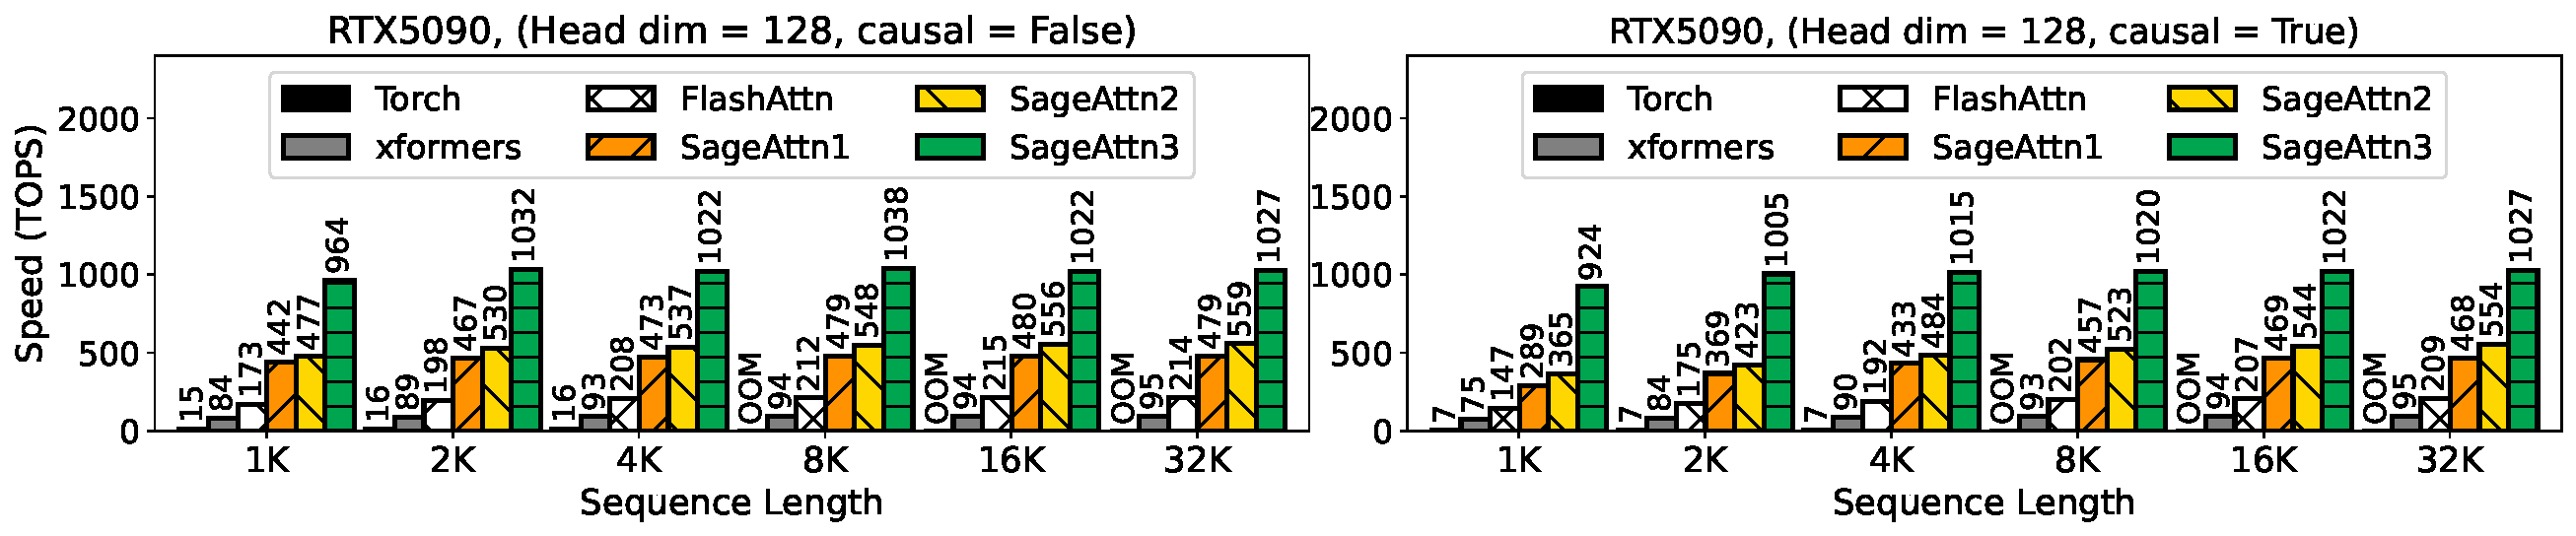
\includegraphics[width=\columnwidth]{src/figs/sage_attn3_hd128_baselines_kernel_flops.pdf} 
    \vspace{-1.5em}
    \caption{Speed comparison between \our and Baselines (\texttt{RTX5090}, headim=128).}
    \vspace{-1em}
    \label{fig:sage3_h128_speed} 
\end{figure}
    
    
\begin{figure}[H]
    \centering
    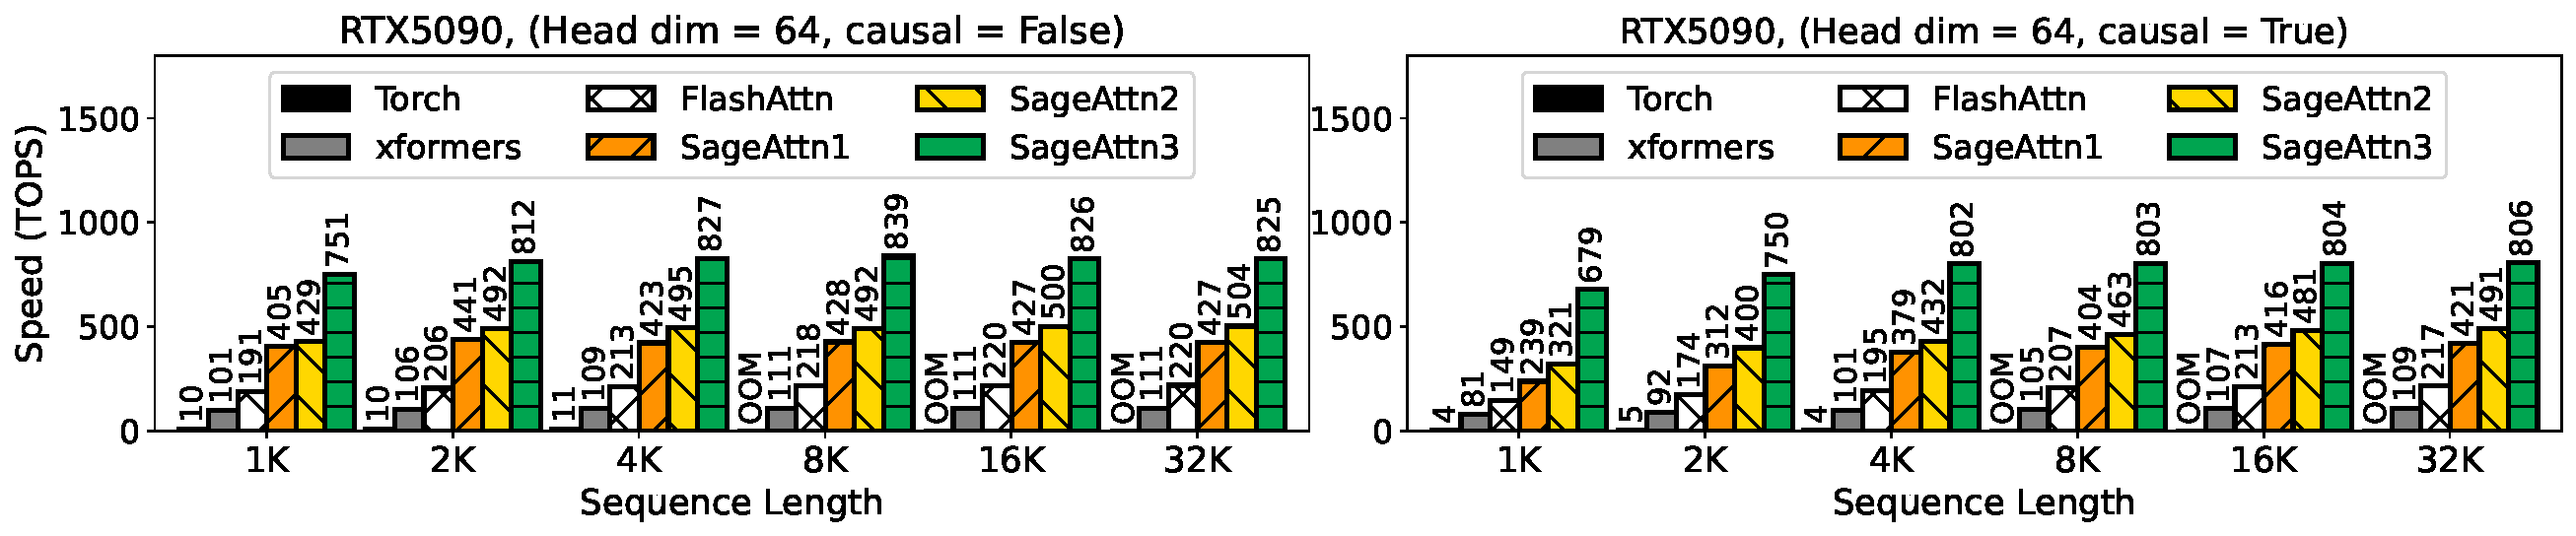
\includegraphics[width=\columnwidth]{src/figs/sage_attn3_hd64_baselines_kernel_flops.pdf} 
    \vspace{-1.5em}
    \caption{Speed comparison between \our and Baselines (\texttt{RTX5090}, headim=64).}
    \vspace{-1em}
    \label{fig:sage3_h64_speed} 
\end{figure}

\begin{figure}[H]
  \centering
  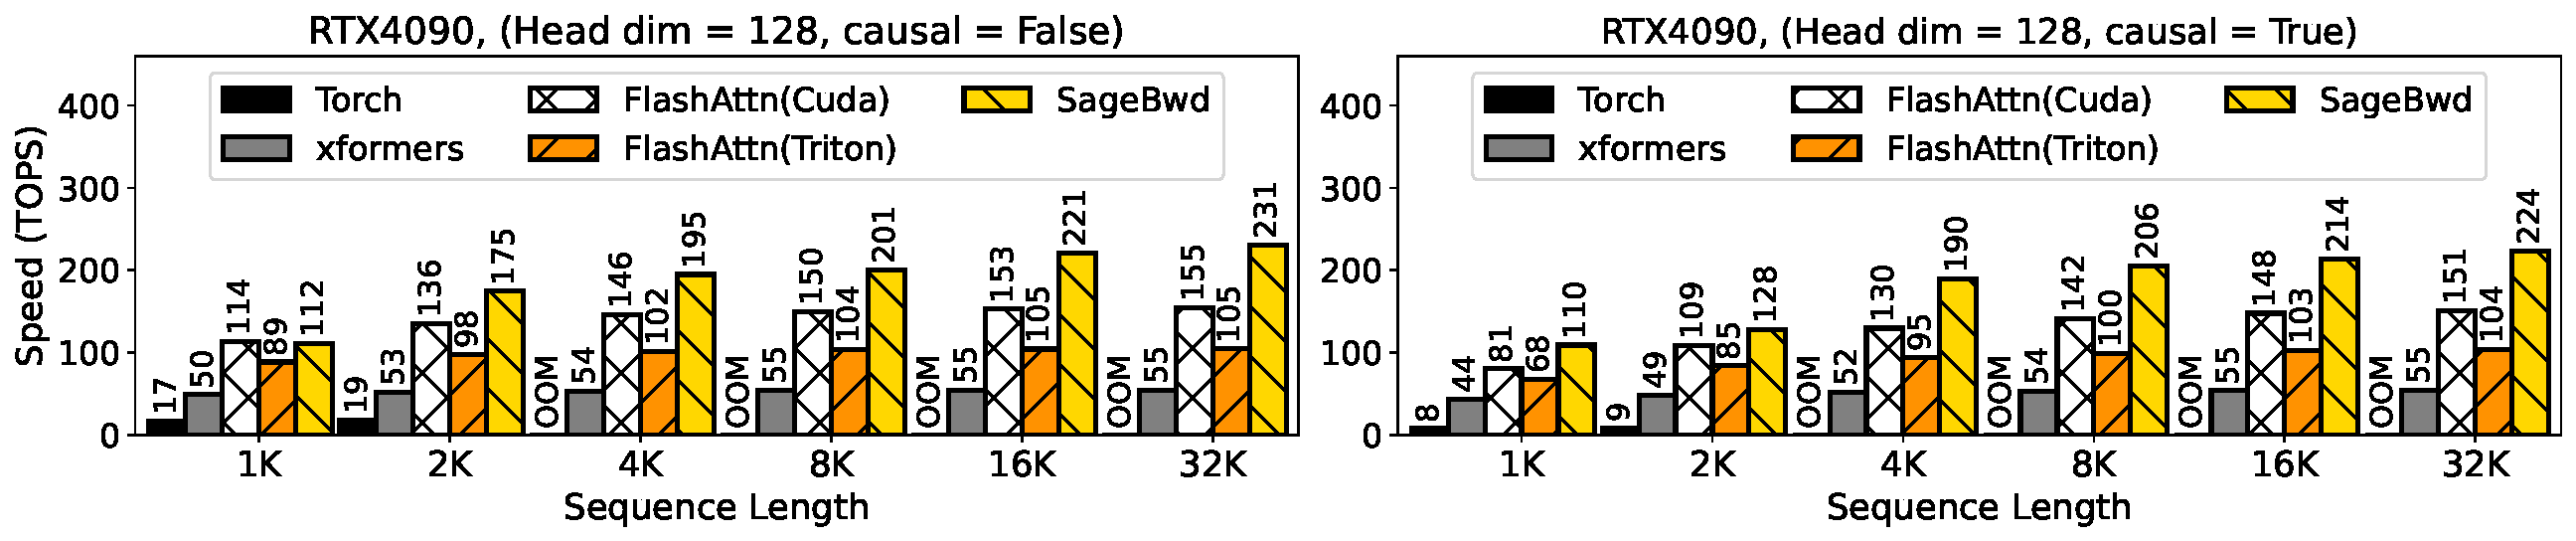
\includegraphics[width=\columnwidth]{src/figs/sage_attn_train_hd128_baselines_kernel_flops.pdf} 
  \vspace{-1.5em}
  \caption{Speed comparison between \texttt{SageBwd} and Baselines (\texttt{RTX4090}, headim=128).}
  \vspace{-1em}
  \label{fig:sage_train_h128_speed} 
\end{figure}

\begin{figure}[H]
    \centering
    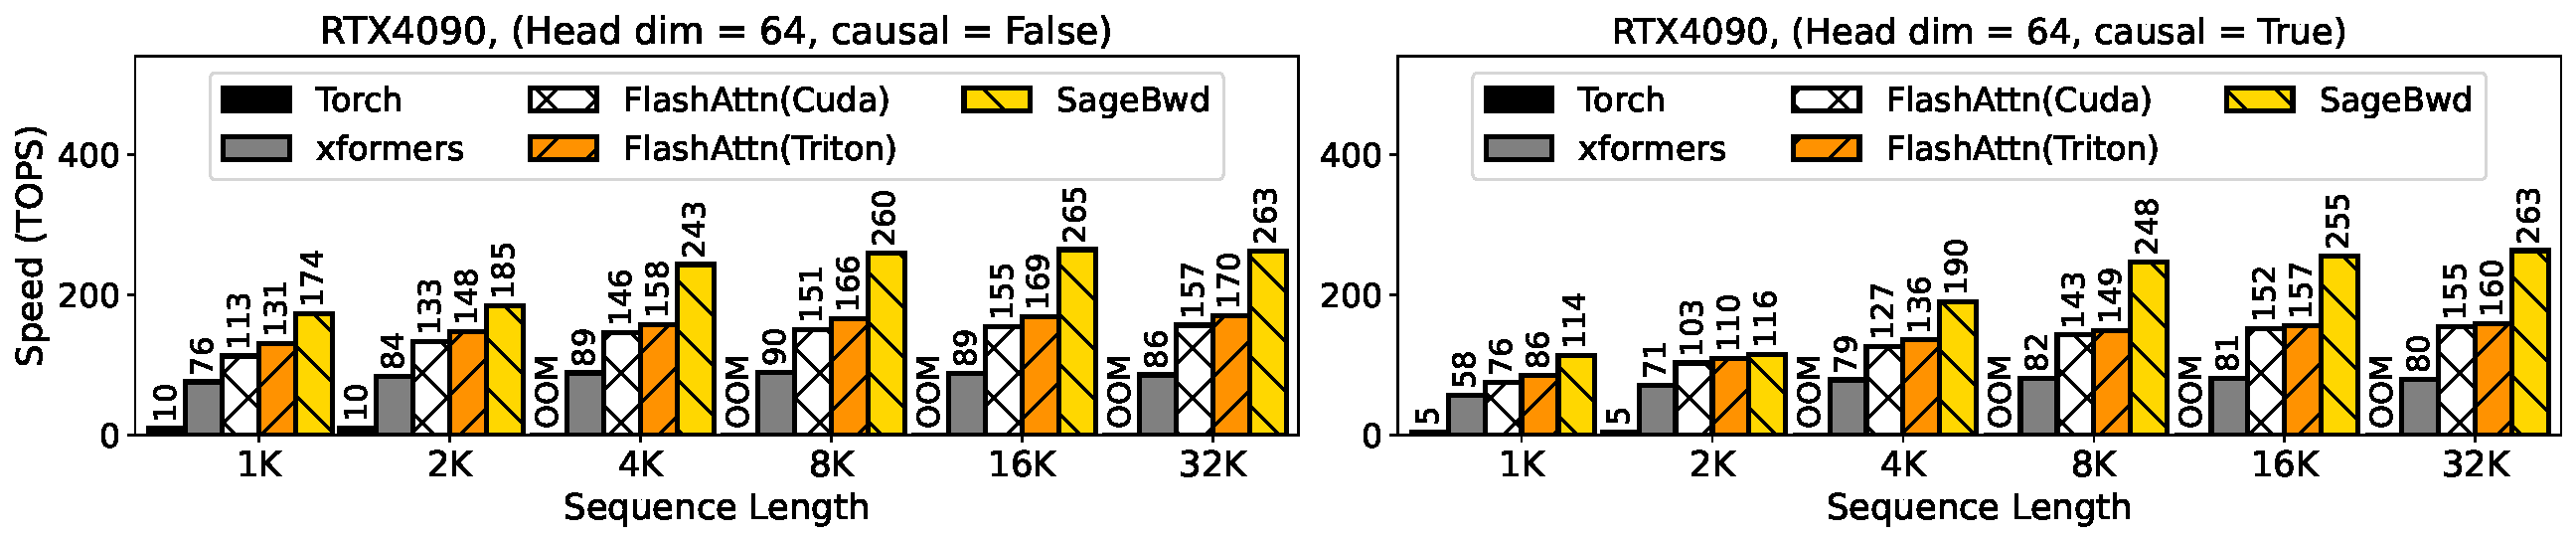
\includegraphics[width=\columnwidth]{src/figs/sage_attn_train_hd64_baselines_kernel_flops.pdf}
    \vspace{-1.5em}
    \caption{Speed comparison between \texttt{SageBwd} and Baselines (\texttt{RTX4090}, headim=64).}
    \vspace{-1em}
    \label{fig:sage_train_h64_speed} 
\end{figure}





\begin{table}[H]  
\vspace{-1em}
        \caption{End-to-end metrics comparison on various models.}
        \sisetup{detect-weight=true, detect-family=true}
        \sisetup{table-auto-round=true}
        \label{tab:end2end_metric}
        \begin{center}
        \setlength\tabcolsep{7pt}
        \scalebox{0.89}{\begin{tabular}{p{1.3cm}
                                        p{3.5cm}
                                        c
                                        c
                                        c
                                        c
                                        c}
        \toprule
        {\bf Model}  & {\mbox{\hspace{2em}\textbf{Attention}}}  & {\bf CLIPSIM $\uparrow$}  & {\bf CLIP-T $\uparrow$}  & {\bf VQA-a $\uparrow$}  & {\bf VQA-t $\uparrow$}  & {\bf FScore $\uparrow$} \\ \hline
    
        \multirow{3}{*}{\mbox{\hspace{-.75em}\makecell[c]{\cogvideo}}} 
& \mbox{\hspace{-.63em}Full-Precision \texttt{(16bit)}}  & 0.1865 & 0.9968 & 70.476 & 69.875 & 4.780 \\
% & \mbox{\hspace{-.63em}\texttt{SageAttention2 (6bit)}}  &  &  &  &  &  \\
& \mbox{\hspace{-.63em}\texttt{SageAttention2 (8bit)}}  & 0.1880 & 0.9969 & 69.414 & 70.750 & 4.534 \\
& \mbox{\hspace{-.63em}\ourf \texttt{(4bit)}}  & \textbf{0.1881} & \textbf{0.9969} & \textbf{69.860} & \textbf{70.364} & \textbf{4.035} \\



         \hline

        \multirow{3}{*}{\mbox{\hspace{-.3em}\makecell[c]{\texttt{Hunyuan}\\ \texttt{Video}}}} 
        & \mbox{\hspace{-.63em}Full-Precision \texttt{(16bit)}}  & 0.1838 & 0.9993 & 68.998 & 78.891 & 1.4793 \\ 
        % & \mbox{\hspace{-.63em}\texttt{SageAttention2 (6bit)}}  &  &  &  &  &  \\
        & \mbox{\hspace{-.63em}\texttt{SageAttention2 (8bit)}}  & 0.1836 & 0.9993 & 69.497 & 77.019 & 1.4741 \\
        & \mbox{\hspace{-.63em}\ourf \texttt{(4bit)}}  & \textbf{0.1866} & \textbf{0.9993} & \textbf{70.552} & \textbf{75.440} & \textbf{1.232} \\ 
        \hline

        \multirow{3}{*}{\mbox{\hspace{.1em}\makecell[c]{\mochi}}} 
        & \mbox{\hspace{-.63em}Full-Precision \texttt{(16bit)}}  & 0.1828 & 0.9990 & 61.9840 & 61.0000 & 1.8042 \\ 
        % & \mbox{\hspace{-.63em}\texttt{SageAttention2 (6bit)}}  &  &  &  &  &  \\
        & \mbox{\hspace{-.63em}\texttt{SageAttention2 (8bit)}}  & 0.1819 & 0.9990 & 61.0093 & 60.3732 & 1.7539 \\
        & \mbox{\hspace{-.63em}\ourf \texttt{(4bit)}}  & \textbf{0.1800} & \textbf{0.9993} & \textbf{61.863} & \textbf{59.429} & \textbf{1.649} \\ 
        \bottomrule

        \end{tabular} }
        \end{center}
    
    \vspace{-.75em}
    
        \begin{center}
        \setlength\tabcolsep{19.45pt}
        \scalebox{0.89}{\begin{tabular}{p{0.51cm}
                                        p{2.6cm}
                                        c
                                        c
                                        c
                                        c}
        \toprule
        {\mbox{\hspace{-.75em}\textbf{Model}}}  & {\bf Attention}  & {\bf FID $\downarrow$}  & {\bf sFID $\downarrow$}  & {\bf CLIP $\uparrow$}  & {\bf IR $\uparrow$}
        \\ \hline

        \multirow{3}{*}{\hspace{-1em}\flux} 
        & \mbox{\hspace{-1.8em}Full-Precision \texttt{(16bit)}} & 162.812 & 146.980 & 31.409 & 0.91 \\ 
        & \mbox{\hspace{-1.8em}\texttt{SageAttention2 (8bit)}} & 163.107 & 146.213 & 31.436 & 0.90 \\
        & \mbox{\hspace{-1.8em}\our \texttt{(4bit)}} & \textbf{162.121} & \textbf{142.839} & \textbf{31.450} & \textbf{0.94} \\
        \hline

        \multirow{3}{*}{\hspace{-2.1em}\texttt{\makecell[c]{Stable-Di\\ffusion3.5}}} 
        & \mbox{\hspace{-1.8em}Full-Precision \texttt{(16bit)}} & 166.421 & 146.379 & 31.93 & 0.93 \\ 
        & \mbox{\hspace{-1.8em}\texttt{SageAttention2 (8bit)}} & 164.986 & 148.557 & 32.01 & 0.93 \\
        & \mbox{\hspace{-1.8em}\ourf \texttt{(4bit)}} & \textbf{166.102} & \textbf{145.587} & \textbf{32.01} & \textbf{0.92} \\
 
        \bottomrule
    \end{tabular} }
    \end{center}
    \vspace{-.5em}
\end{table}


\begin{figure}[H]
\vspace{-1em}
  \centering
  \begin{minipage}[b]{0.19\textwidth}
    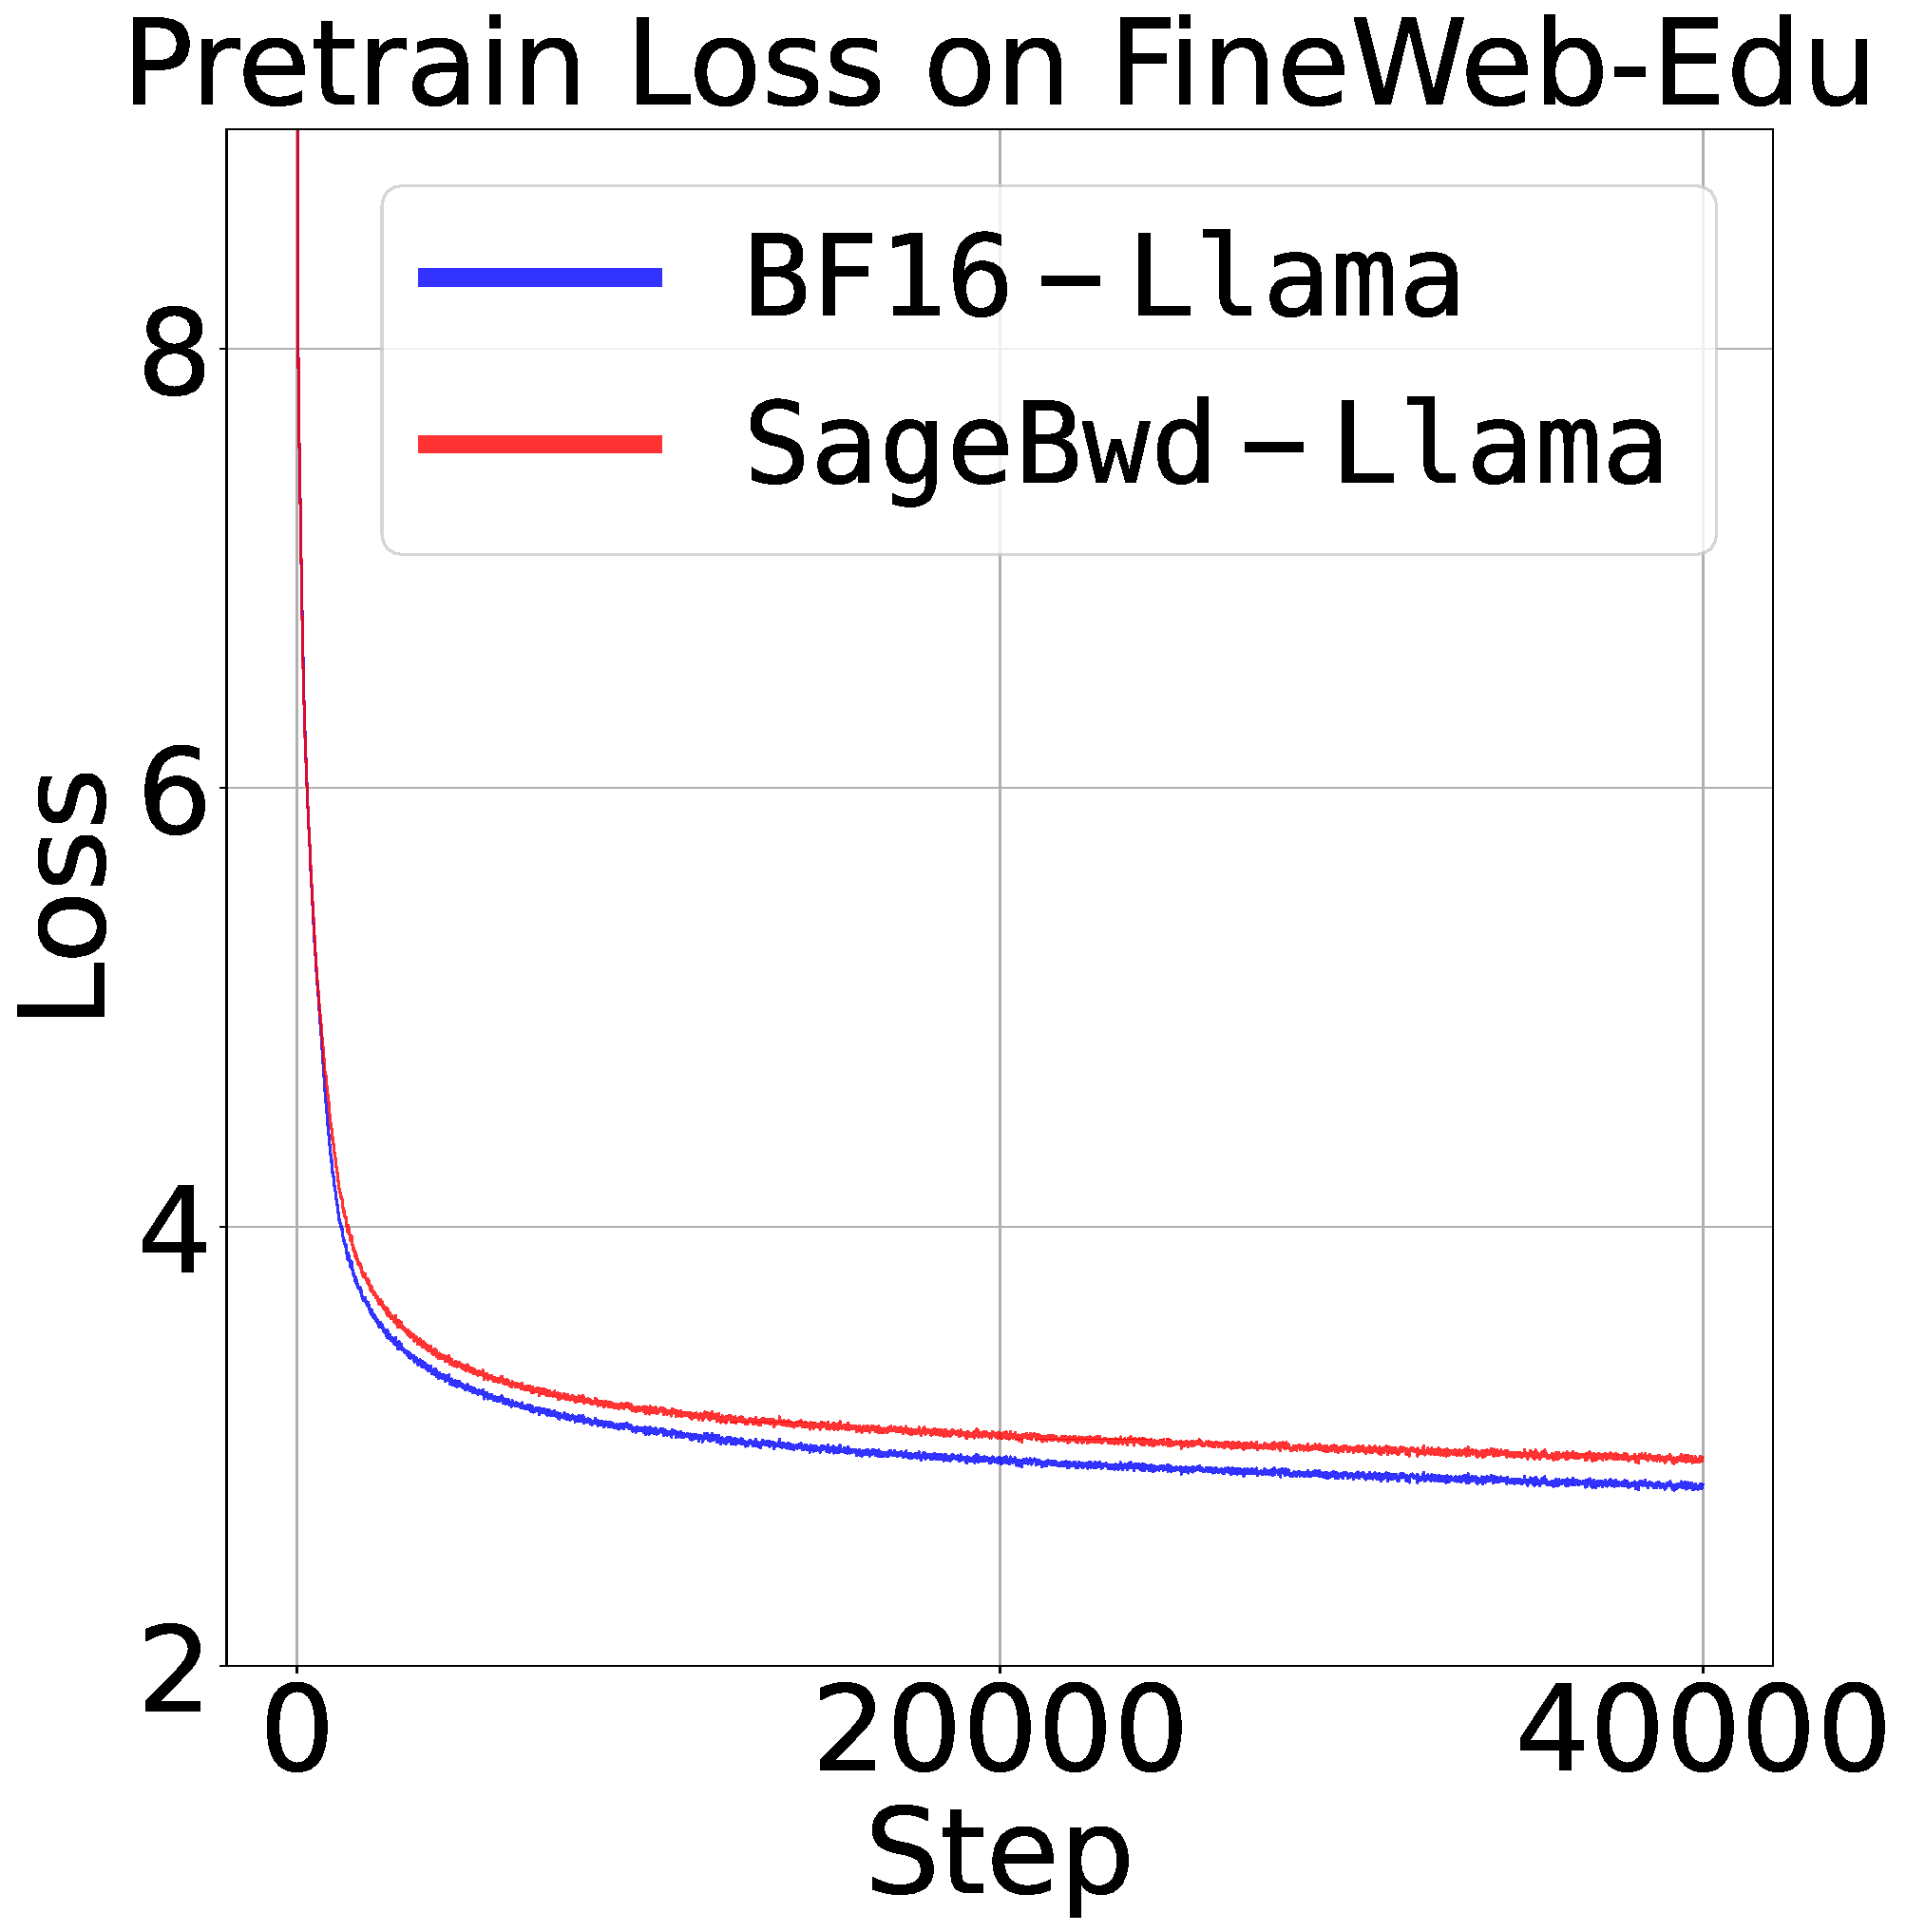
\includegraphics[width=\linewidth]{src/figs/pretrain-loss.pdf}
    \subcaption{}
    \label{fig:train_a}
  \end{minipage}
  \begin{minipage}[b]{0.187\textwidth}
    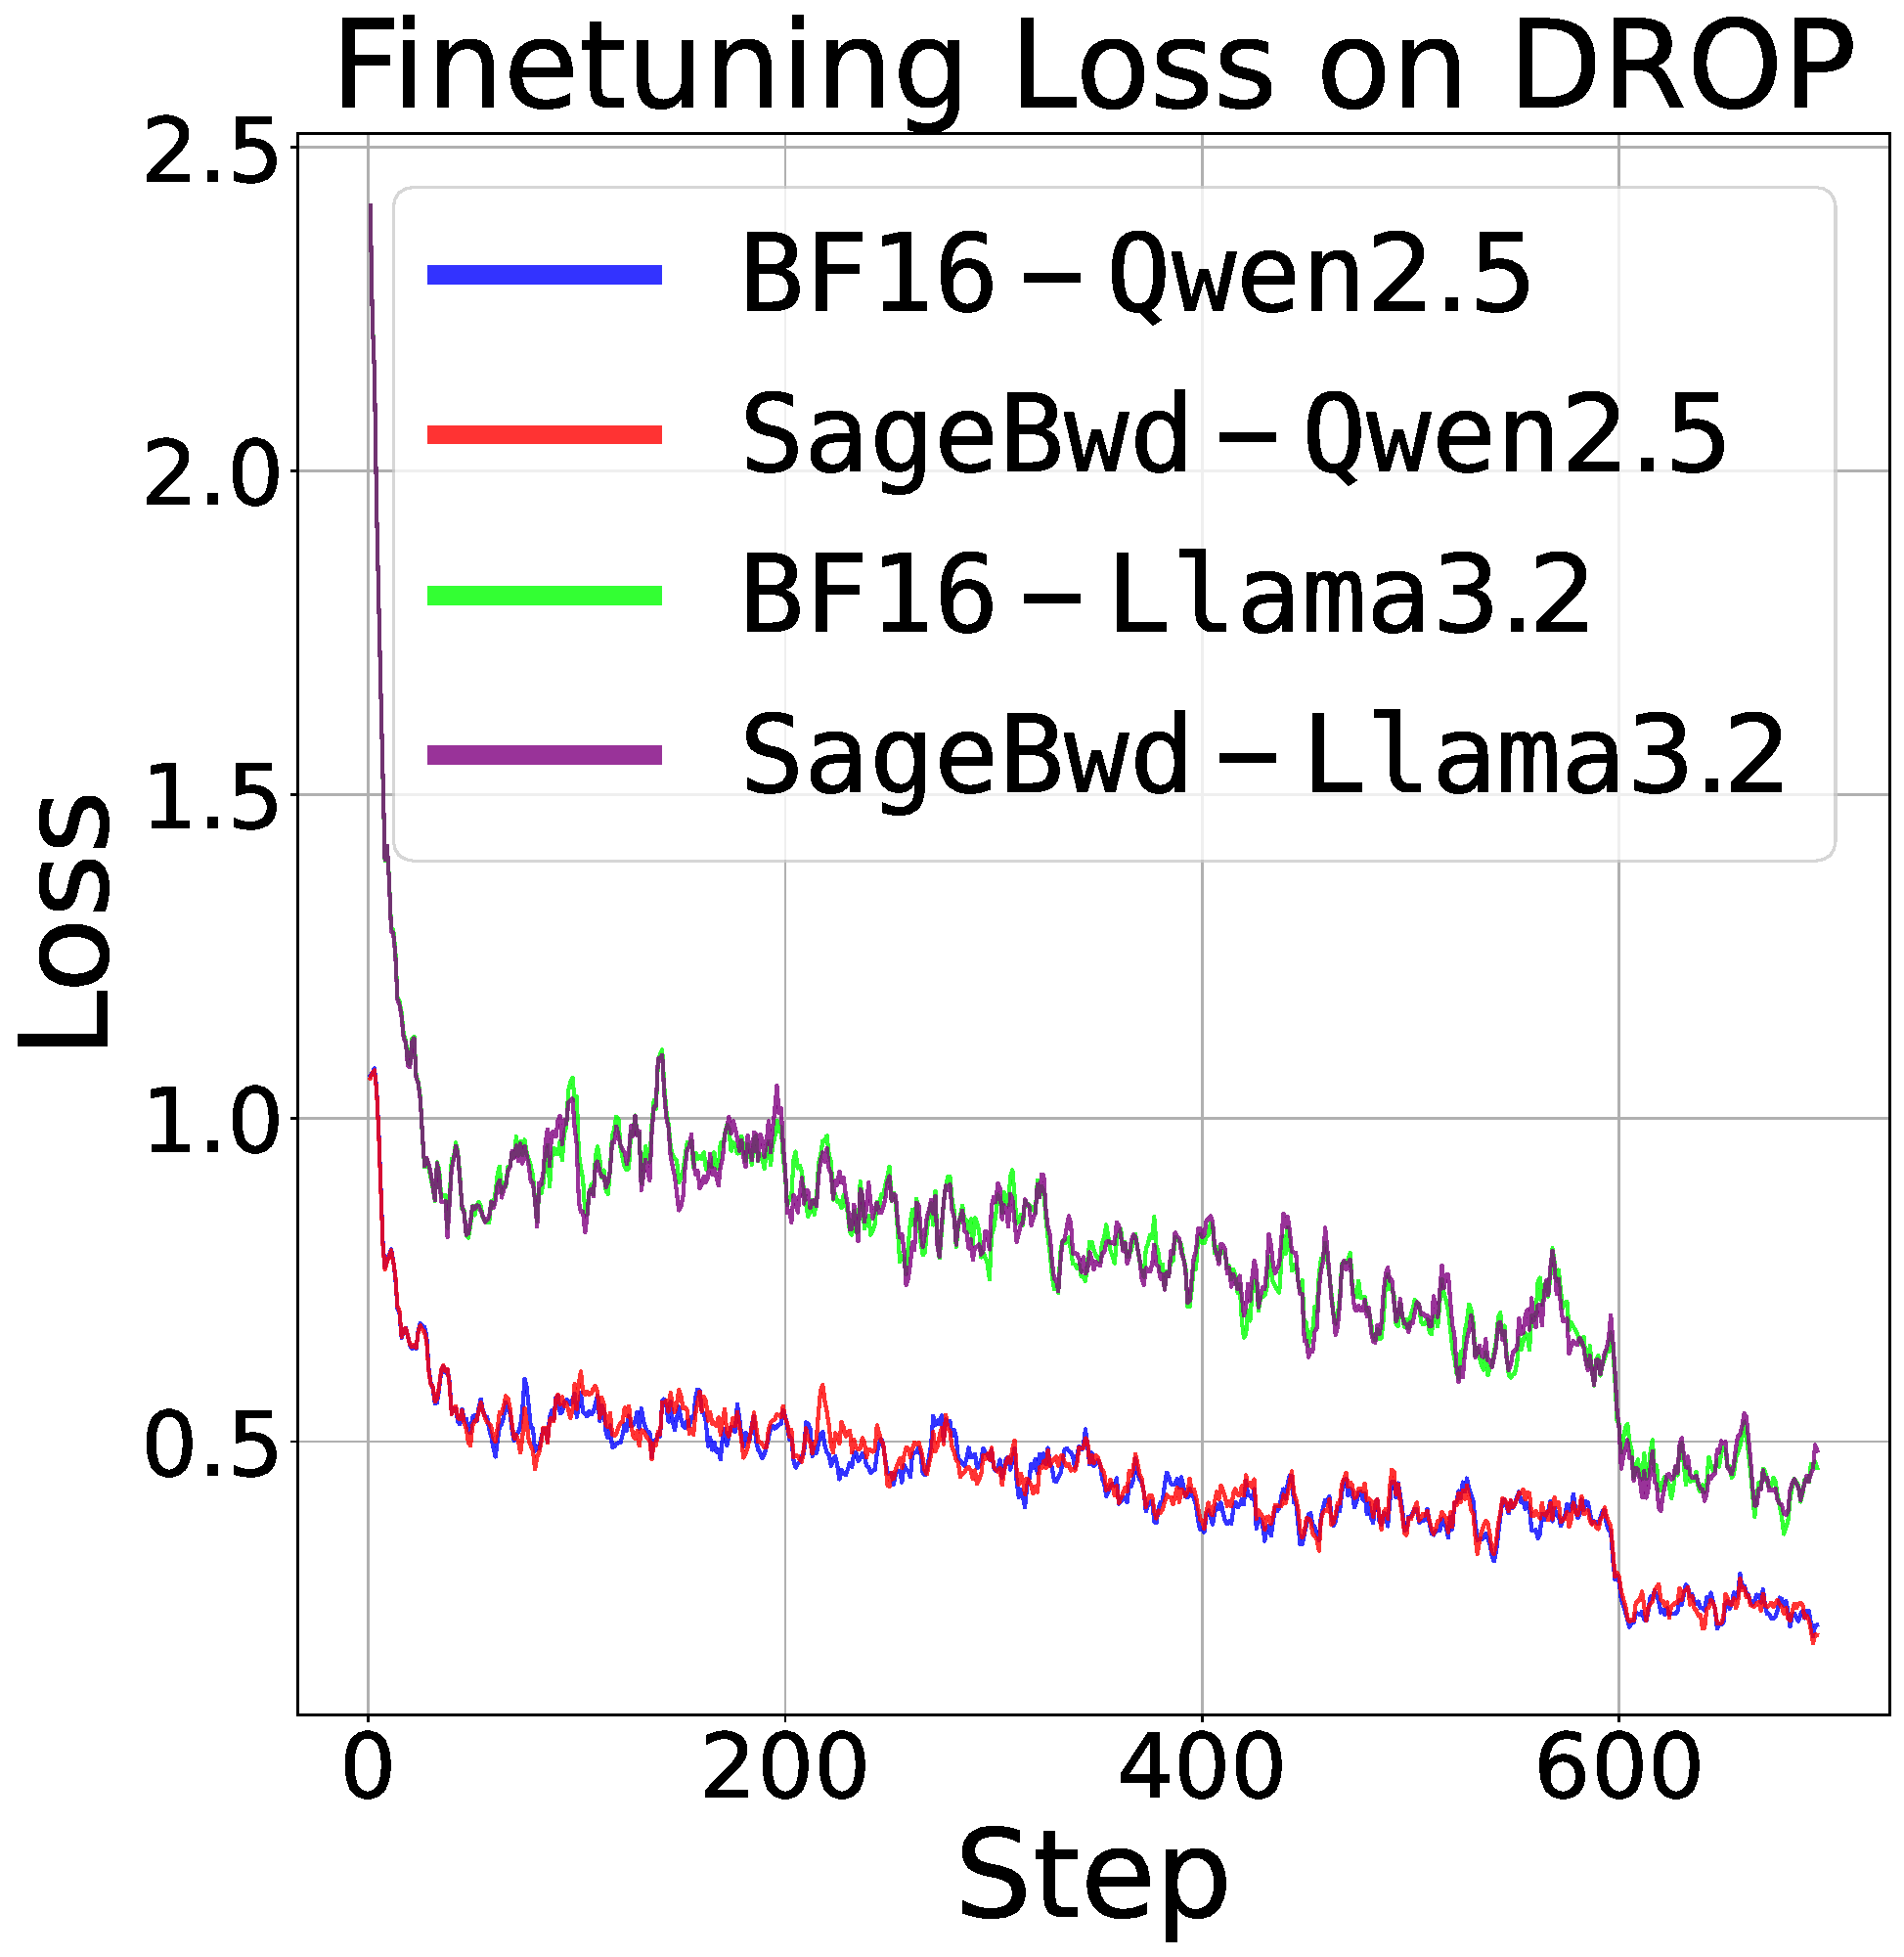
\includegraphics[width=\linewidth]{src/figs/finetune-drop-loss.pdf}
    \subcaption{}
    \label{fig:train_b}
  \end{minipage}
  \begin{minipage}[b]{0.193\textwidth}
    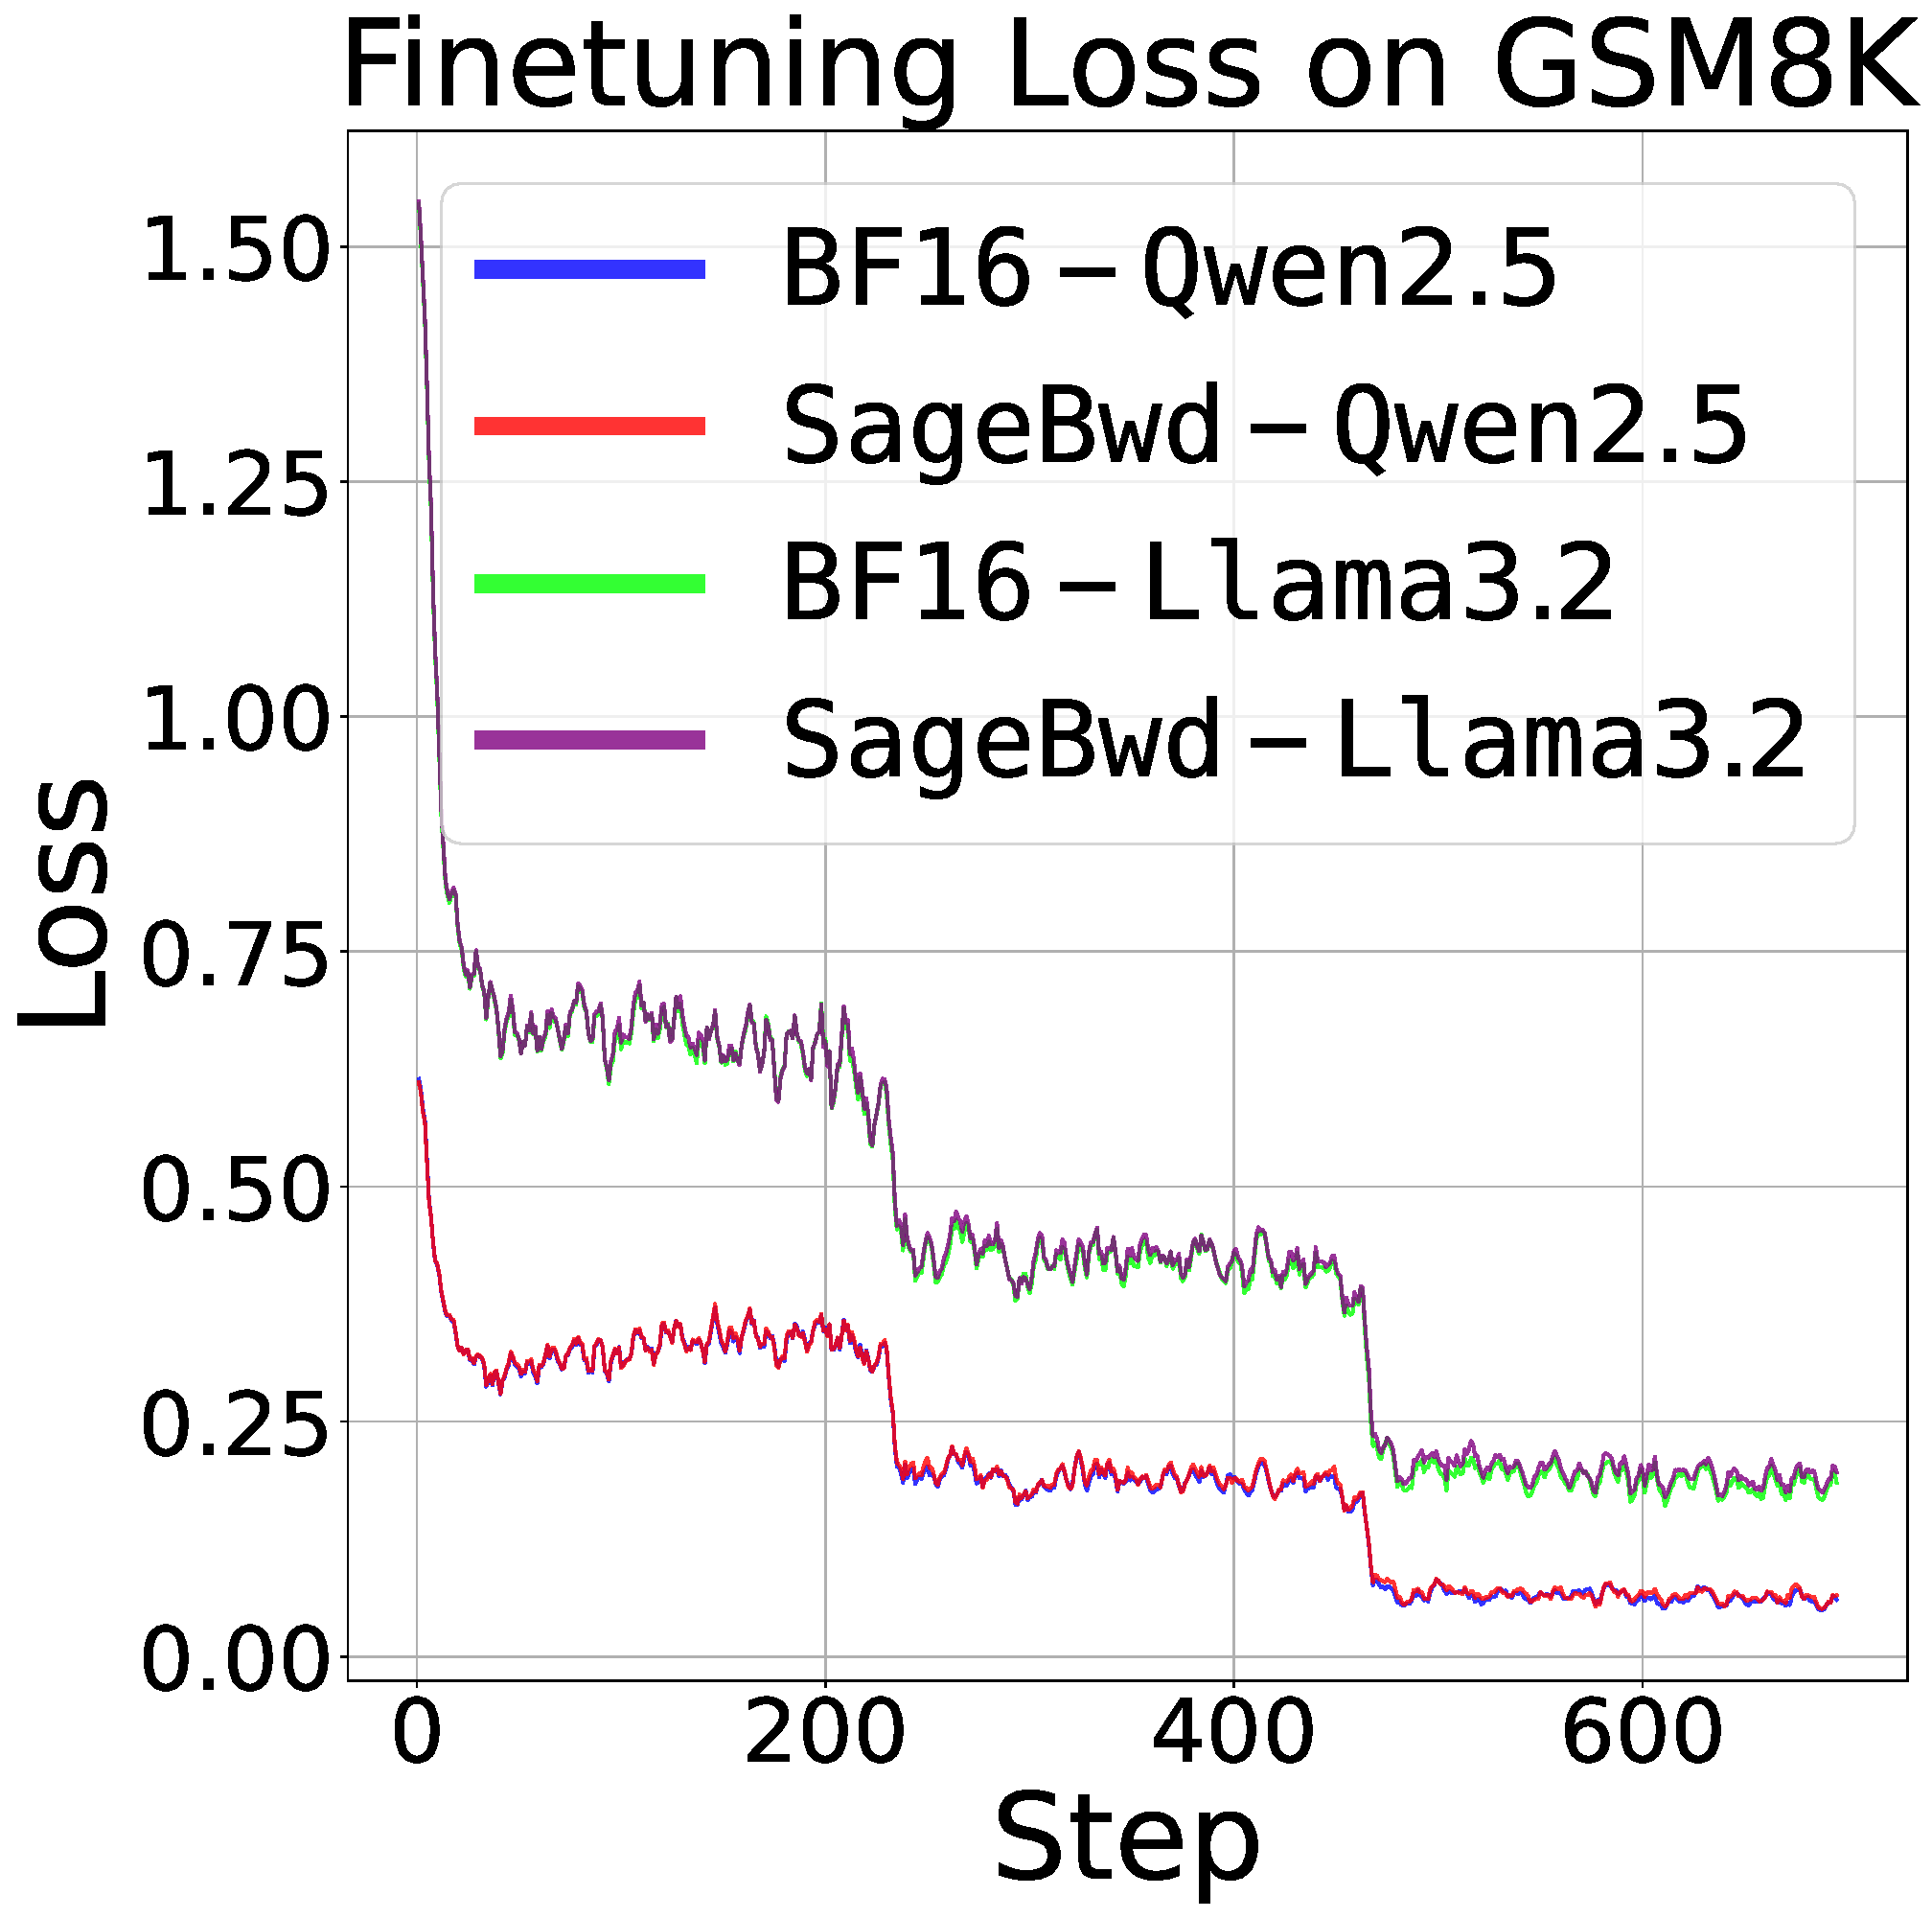
\includegraphics[width=\linewidth]{src/figs/finetune-gsm8k-loss.pdf}
    \subcaption{}
    \label{fig:train_c}
  \end{minipage}
  \begin{minipage}[b]{0.203\textwidth}
    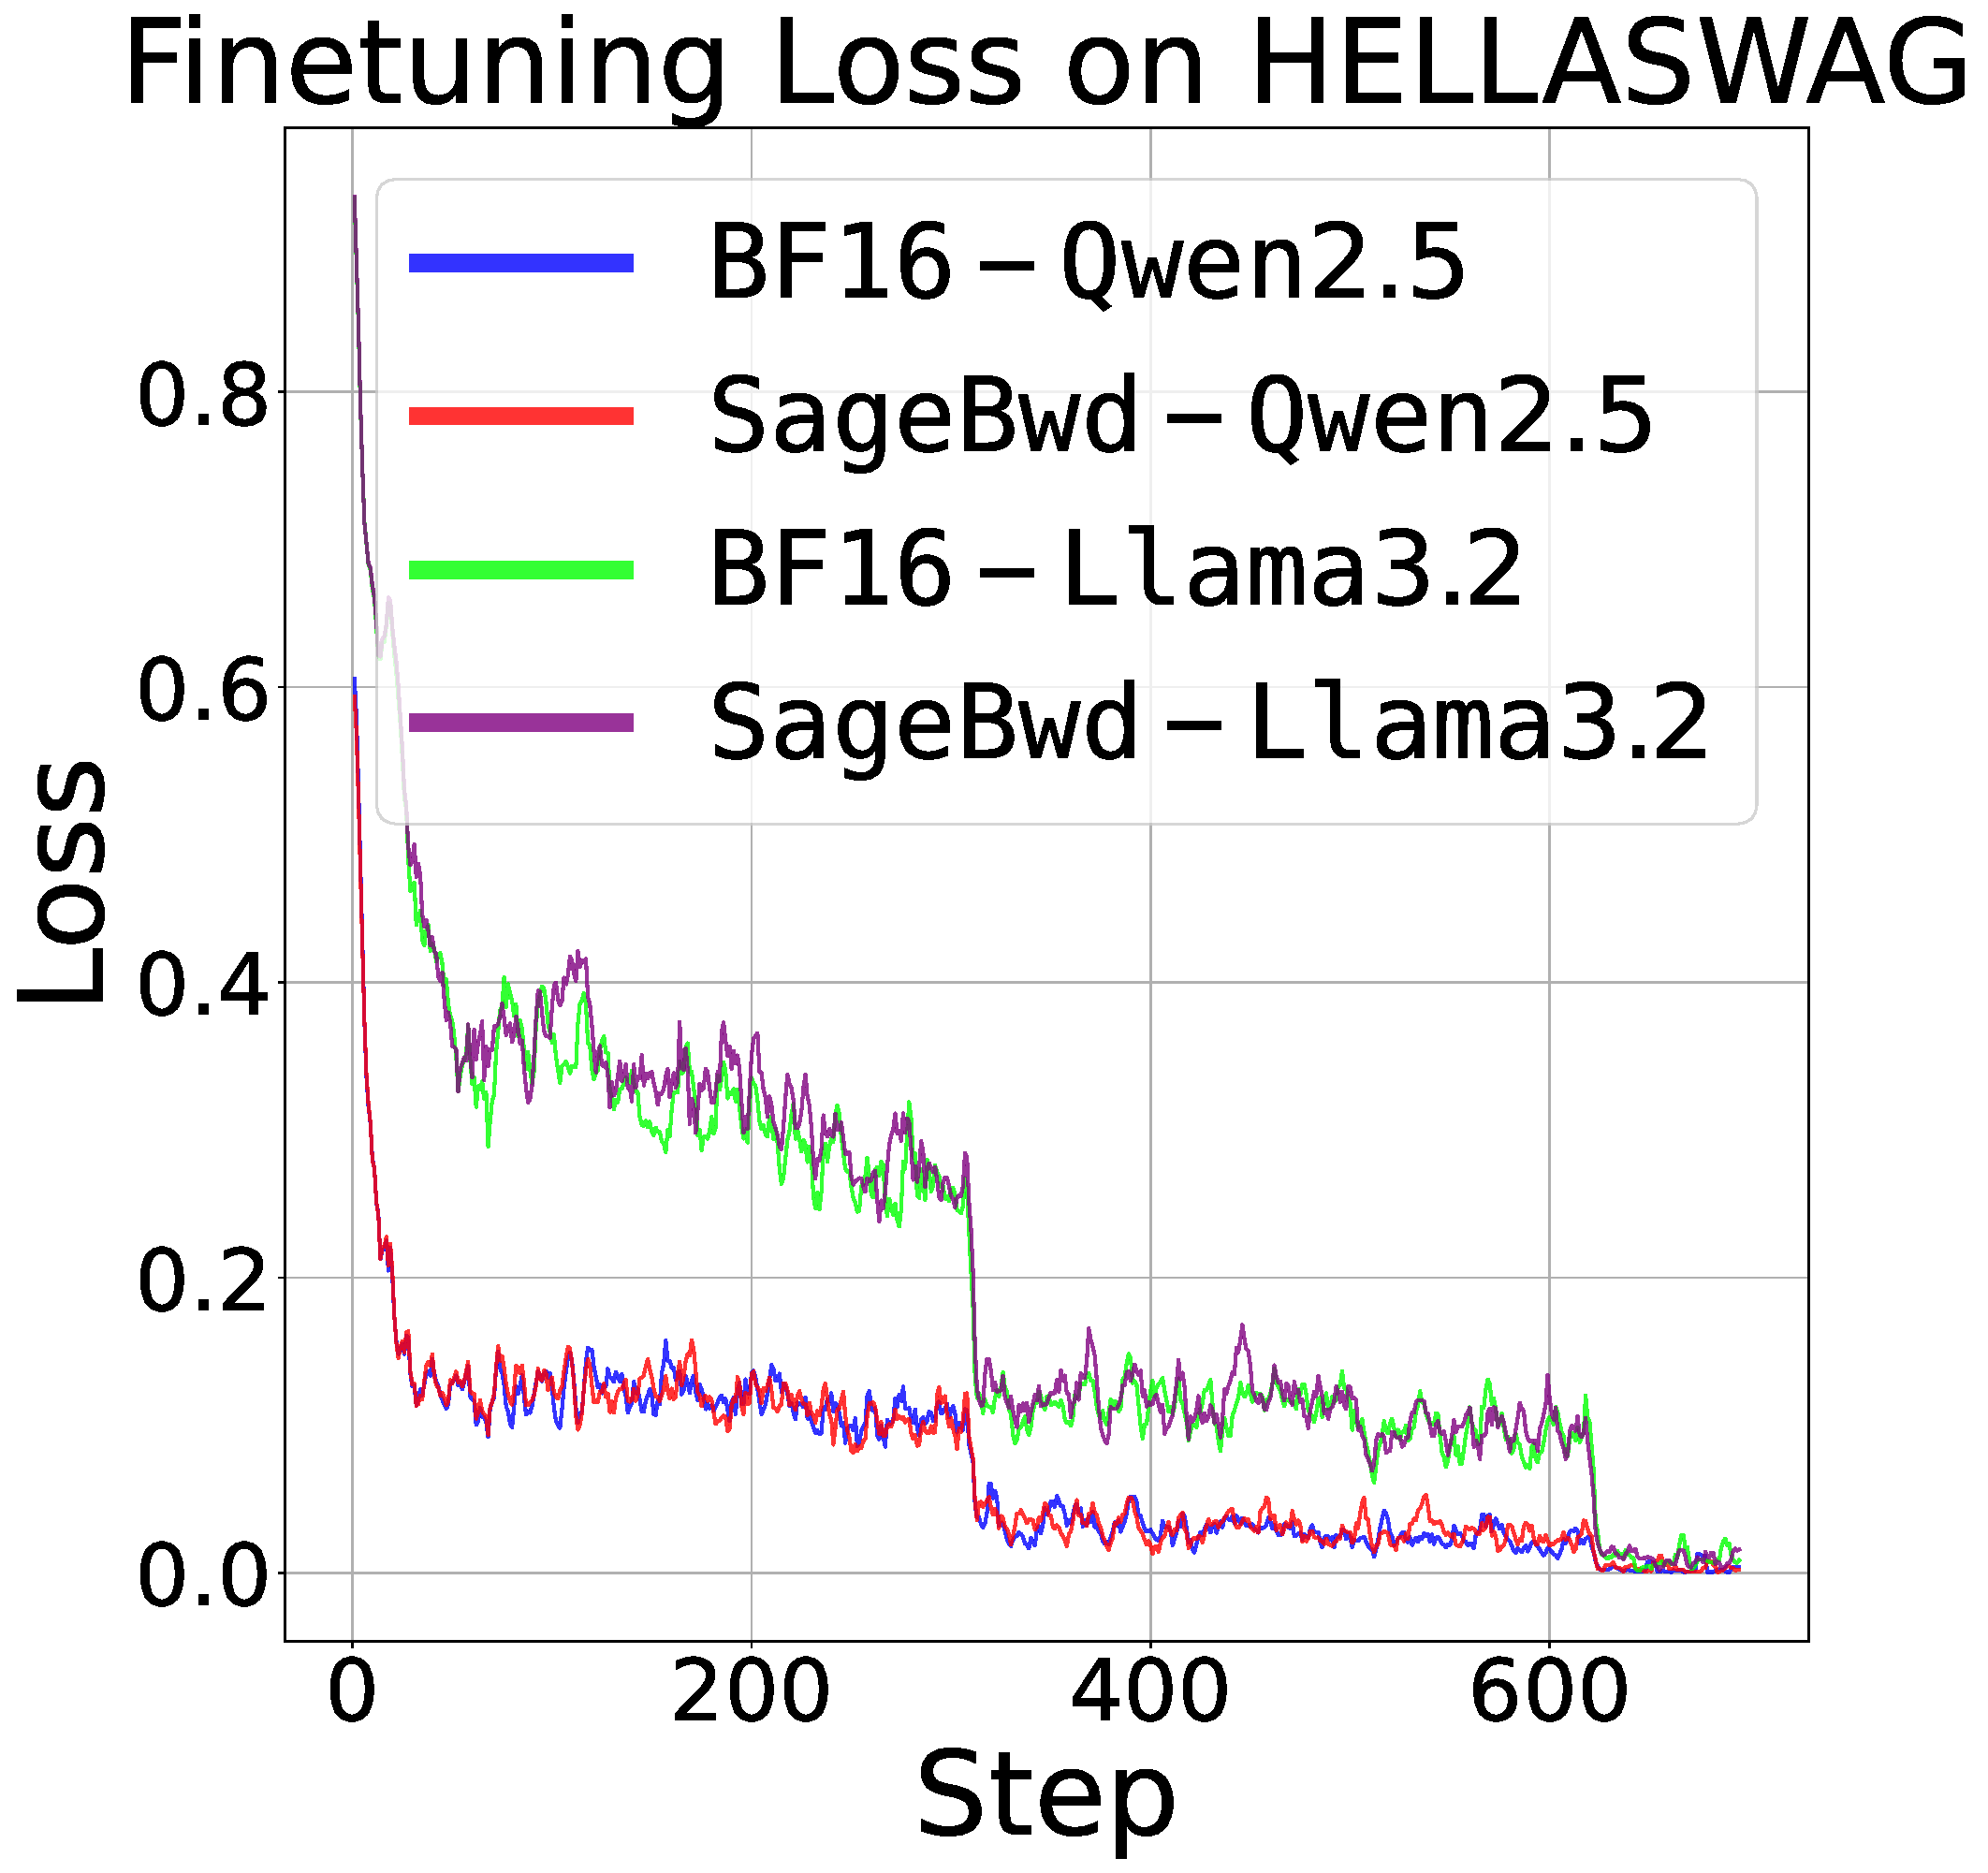
\includegraphics[width=\linewidth]{src/figs/finetune-hellaswag-loss.pdf}
    \subcaption{}
    \label{fig:train_d}
  \end{minipage}
  \begin{minipage}[b]{0.187\textwidth}
    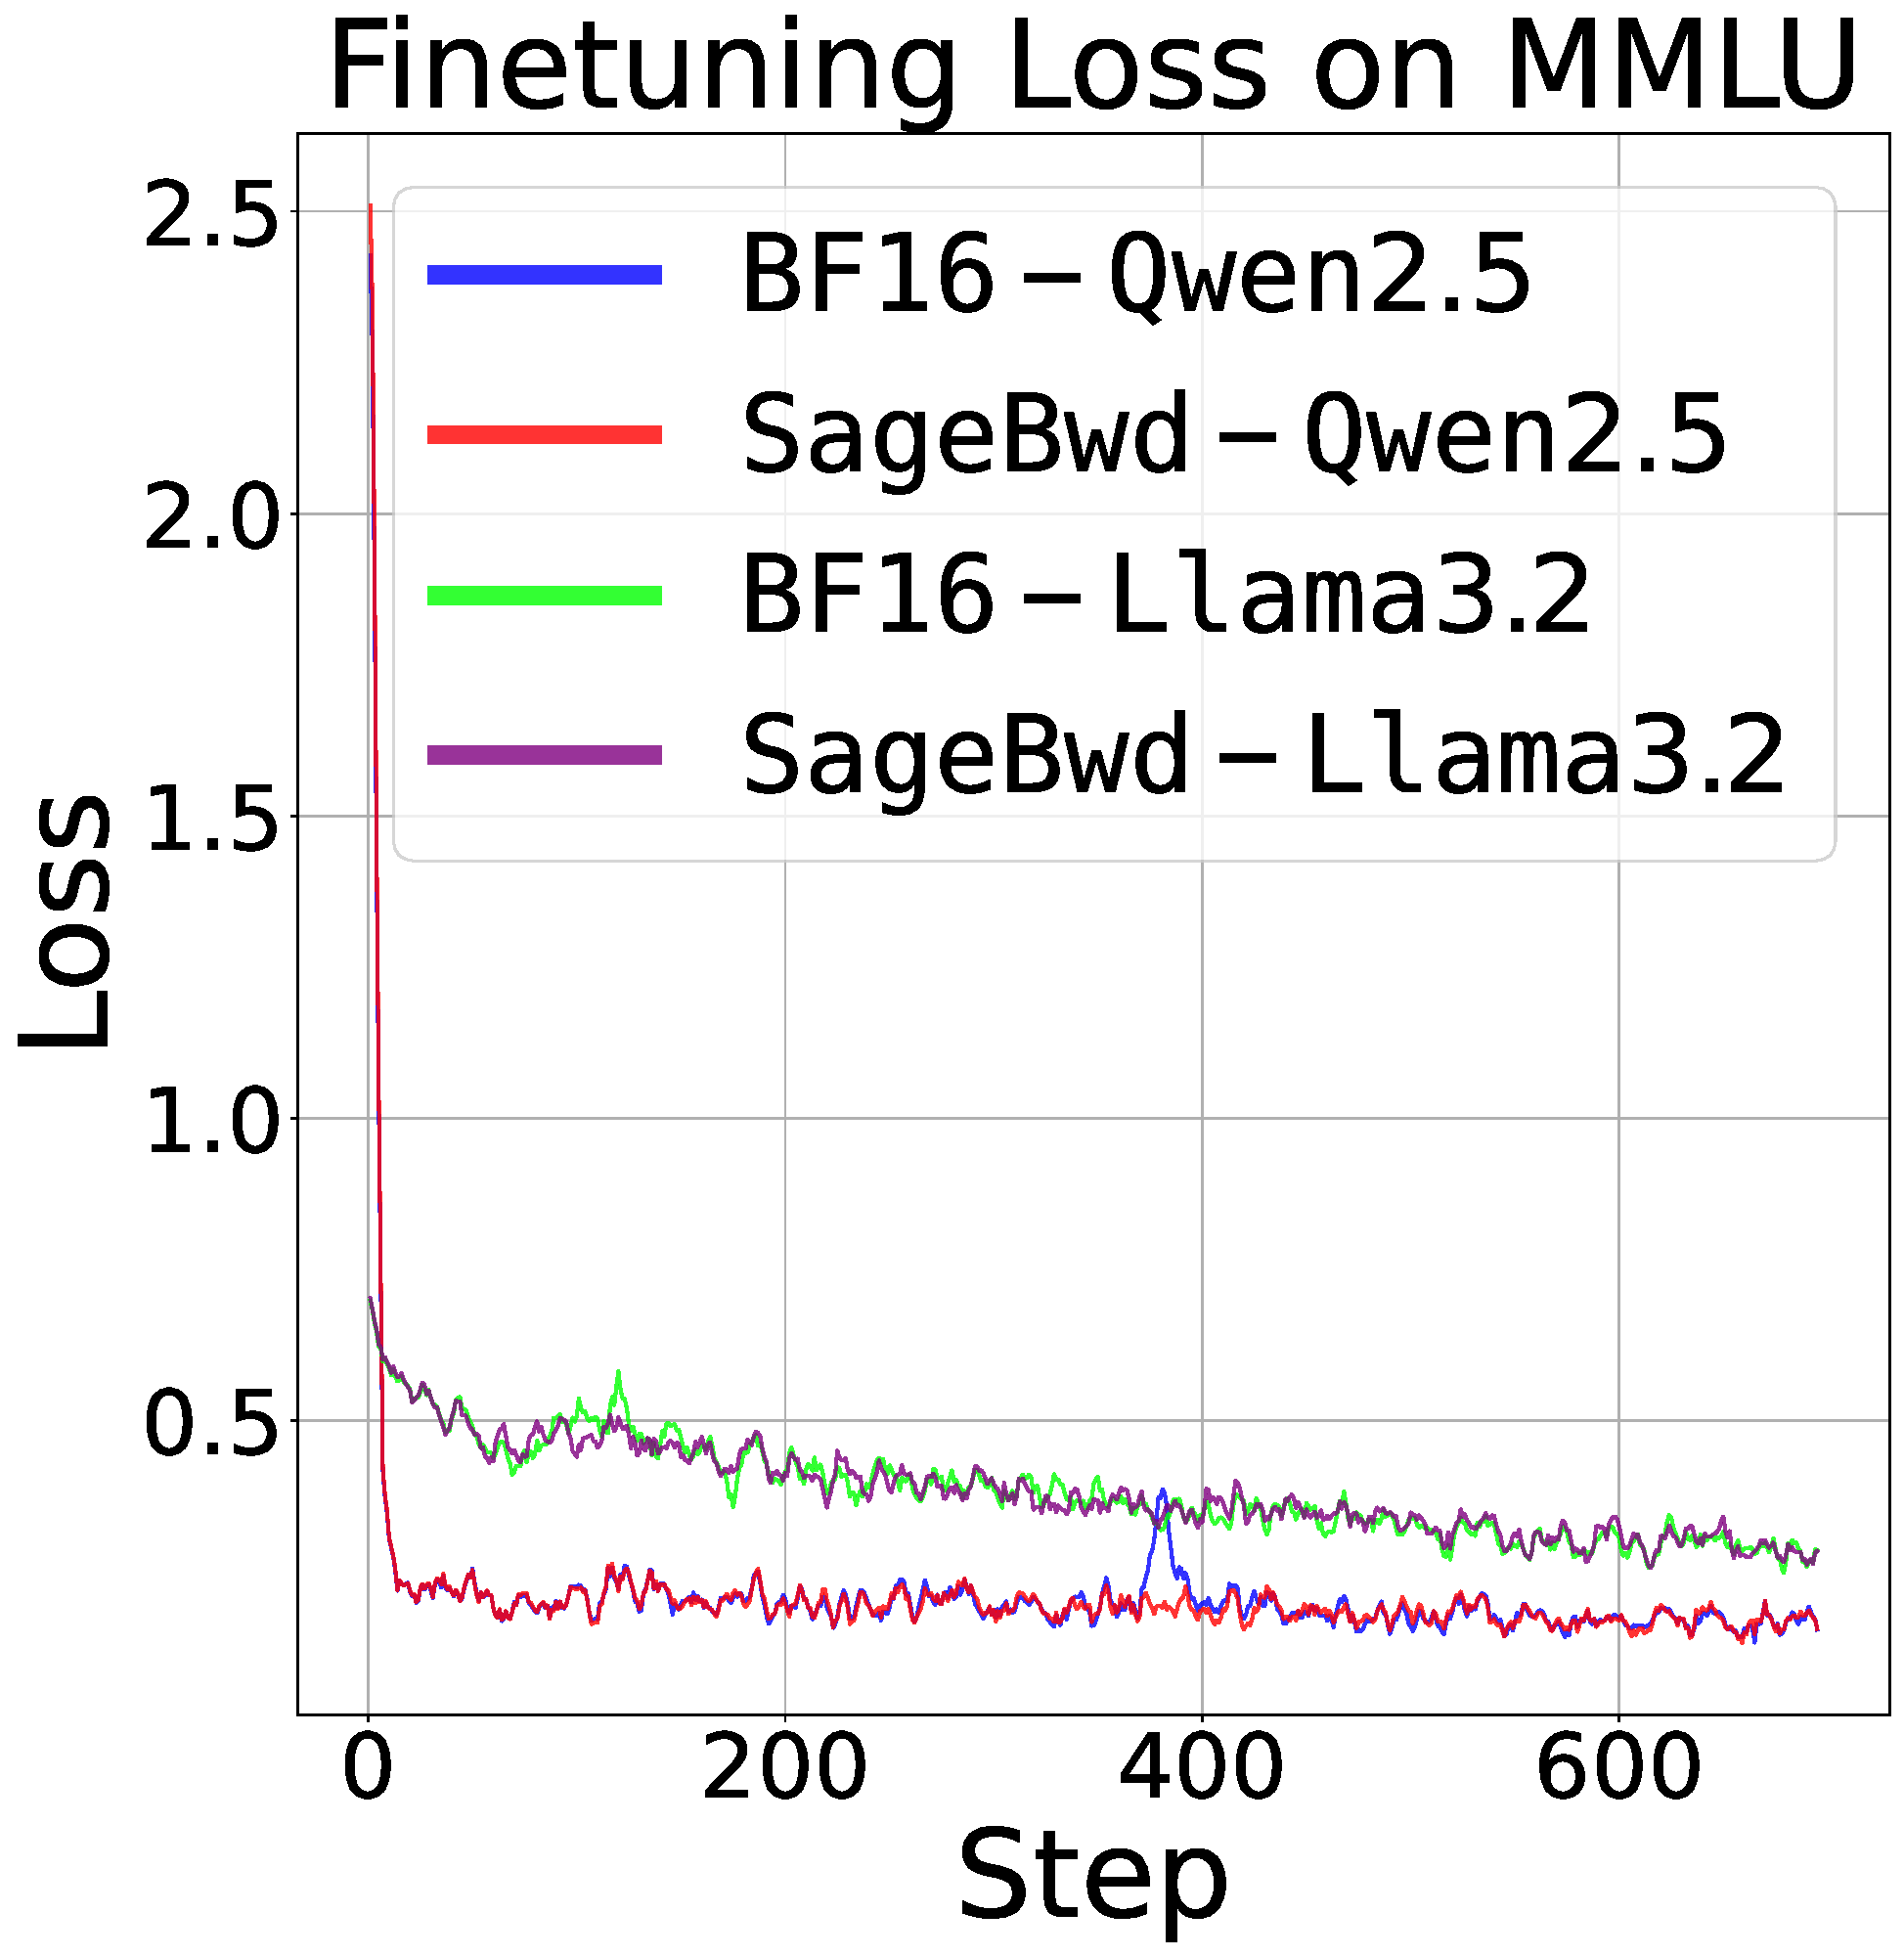
\includegraphics[width=\linewidth]{src/figs/finetune-mmlu-loss.pdf}
    \subcaption{}
    \label{fig:train_e}
  \end{minipage}
  \vspace{-.45em}
  \caption{Pretraining and Finetuing loss curves of \texttt{BF16} and \texttt{8-bit} atttention.}
  \vspace{-.5em}
  \label{fig:finetune-loss}
\end{figure}



\begin{table}[H] 
% \small
\centering
\caption{\texttt{8-bit} attention finetune results on \qwen and \llamal models.}
\label{tab:finetune}
% \scriptsize
\scalebox{0.96}{
\begin{tabular}{
    cc 
    cc
    cc
    cc
    cc
    cc
}
\toprule
{Model} 
& {Method} 
& {GSM8K}\tiny{(Acc$\uparrow$)} 
& {DROP}\tiny{(F1$\uparrow$)}
& {MMLU}\tiny{(Acc$\uparrow$)} 
& {HELLASWAG}\tiny{(Acc$\uparrow$)} \\
\midrule
\multirow{2}{*}{\qwen(1.5B)} & \texttt{BF16} 
& 0.521 & 0.733 & 0.569 & 0.905 \\
\cmidrule{2-6}
& \texttt{SageBwd} 
& 0.520 & \textbf{0.734} & \textbf{0.574} & \textbf{0.911} \\

\midrule
\multirow{2}{*}{\qwen(3B)} & \texttt{BF16} 
& 0.601 & 0.785 & 0.640 & 0.944 \\
\cmidrule{2-6}
& \texttt{SageBwd}  
& \textbf{0.607} & 0.782 & \textbf{0.653} & 0.943 \\

\midrule
\multirow{2}{*}{\llamal(1B)} & \texttt{BF16} 
& 0.259 & 0.641 & 0.464 & 0.828 \\
\cmidrule{2-6}
& \texttt{SageBwd}   
& \textbf{0.268} & 0.637 & 0.458 & 0.823 \\
\bottomrule
\end{tabular}}
% \vspace{-1em}
\end{table}













% \section{SageAttention2++}
% % SageAttention2~\cite{} use FP8 quantization to accelerate the $\widetilde \vP \vV$. However, Xxx. we propose to use the xxx to further accelerate xxx. This method pose a new problem. Specifically, xxx. To address this issue, we xxx. 

% % Specifically, the range of 

% SageAttention2~\cite{} employs FP8 quantization to accelerate the $\widetilde \vP \vV$ computation. It utilizes the (mma.f32.f8.f8.f32) instruction, which uses FP32 matrix multiplication accumulators and achieves twice the speed of FP16 matrix multiplication. To further accelerate the speed of $\widetilde \vP \vV$. We propose to use the (mma.f16.f8.f8.f16) instruction to further accelerate SageAttention2, which provides 4$\times$ speedup than in FP16. However, this approach introduces a new challenge. Specifically, directly using this instruction causes the results of the PV matrix multiplication to overflow the representable range of FP16 accumulators.

% However, this optimization introduces a critical numerical precision challenge: In (mma.f16.f8.f8.f16), $\widetilde \vP \in \mathbb{R}^{16\times 32}$ (range $\mathsf{[0,448]}$) and $\vV \in \mathbb{R}^{32\times 16}$ (range $\mathsf{[-448,448]}$). The resulting matrix product $\widetilde \vP \vV$ exceed the FP16 accumulator's representable range of $\mathsf{[-6.55e4, 6.55e4]}$. We address this overflow by reducing the quantization range of P and V. For example:
% \begin{align}
%     s_{\widetilde P} &= \max(|\widetilde \vP|)/r_P, ~~~ r_P=224.0 \\
%     s_V &= \max(|\vV|)/r_V, ~~~ r_V=9.0
% \end{align}


% Through xxx, xxx. 
% The detailed algorithm is shown in Algorithm~\ref{} in Appendix.


% \section{Disscusion of Other Tricks}

% \subsubsection{Stochastic Quantization}
% Xxx. $\phi (\widetilde P)$.


% \subsubsection{Static Smoothing and Scaling V}
% 1. Q K smoothing in SageAttention2.

% 2. Smoothing V

% 3. Scaling V

